% include the figures path relative to the master file
\graphicspath{ {./content/method/figures/} }
\section{Background}\label{sec:review}
This section reviews works straightly addressing the problem of classifying \gls{oct} volumes as normal or abnormal, regardless of the target pathology.
The methods are categorized in terms of its learning strategy, namely: supervised or semi-supervised.


\subsection{Supervised methods}
% Common framework
% \added[id=mojh]{
%   All the previously mentioned methods follow a similar pipeline or framework, which consists of different steps.
%   We categorized these steps as pre-processing, feature extraction, mapping, feature representation and finally classification, as it is shown in Fig.\,\ref{fig:ML-scheme}.

%   Pre-processing of \gls{oct} volumes, as noted in Sect.\,\ref{sec:review}, consists of denoising, flattening the retinal curvature, aligning the B-scans through the whole volume and finally cropping or resizing the volumes.
%   Feature extraction refers to extraction of different textural and shape information from the B-scan or the volumes.
%   Mapping step is used to determine a discrete set of elements (structures) representing a sample (i.e.B-scan/volume).
%   In this step either one structure is used per sample namely global-mapping or the features are extracted with reference to a set of structures, i.e.dense or sparse patches through the sample, local-mapping.

%   In feature representation step, the representation of the final descriptor prior to classification is decided.
%   The extracted features using different mapping techniques can be represented in lower dimensions (using \gls{pca} for instance), as a concatenated of descriptor, histogram of words (using \gls{bow}) or sparse representation (sparse coding).
% }

Supervised classification is based on full annotated and labeled training set.
In such methods the labeled training data is used to train the classifier function, which is latter used for prediction.
% Semi-supervised classification takes advantage of both unlabeled and labeled data.
% This techniques are particularly useful when there is lack of annotated data moreover it has shown that use of small amount of labeled data in conjunction of unlabeled data can increase the learning accuracy.
%
Figure~\ref{fig:ML-scheme} describes a prevalent structure for supervised classification.
The volumes undergo:
(i) \emph{Pre-processing} to reduce the natural noise of the images and correct acquisition deficiencies;
(ii) \emph{Feature detection} to quantify visual cues like appearance, texture, shape, etc.
(iii) \emph{Mapping} to determine the discrete set of elements (structures) to represent the sample to be classified (i.e.B-scan/volume);
(iv) \emph{Feature representation} to associate a descriptor for each element from the \emph{mapping-stage}.
This descriptor packages the visual cues associated to the sample.
(v) \emph{Classification}.

% The details implementation of the following methods and their integration to our common framework is described in Sect.~\textit{experiments}.

\begin{figure*}
  \centering{
  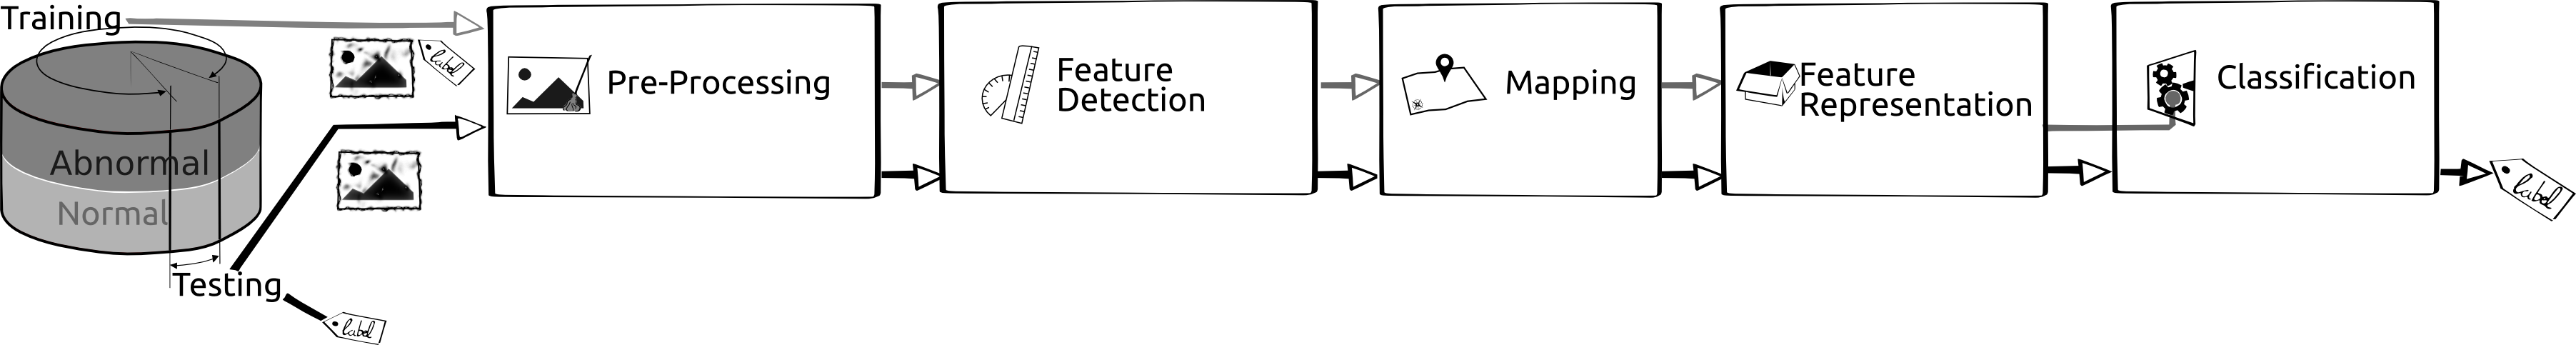
\includegraphics[width=1\linewidth]{ml-2}}
  \caption{Common framework}
  \label{fig:ML-scheme}
\end{figure*}

%%% Venhuizen2015
%
% Brief method description (or goal)
Venhuizen\,\textit{et\,al.} propose a classification method to distinguish between \gls{amd} and normal \gls{sdoct} volumes using \gls{bow} models~\cite{Venhuizen2015}.
%
% Method description
The method detects and selects a set of keypoints at each individual B-scan.
Essentially, keeping the salient points comprised at the top $3\%$ of the vertical gradient values.
Then, a texton of size $9 \times 9$ pixels is extracted around each keypoint, and \gls{pca} is applied to reduce the dimension of every texton to get a feature vector of size $9$.
All extracted feature vectors are used to create a codebook using \textit{k}-means clustering.
Then, each \gls{oct} volume is represented in terms of this codebook and is characterized as a histogram that captures the codebook occurrences.
These histograms are used as feature vector to train a \gls{rf} with a maximum of $100$ trees.
%
% Reported results
The method is tested using a publicly available dataset of $384$ \gls{oct} volumes~\cite{farsiu2014quantitative}, achieving an \gls{auc} of $0.984$.

%%% Srinivasan2014
%
% Brief method description (or goal)
Srinivasan\,\textit{et~al.}~\cite{Srinivasan2014} propose a classification method to distinguish \gls{dme}, \gls{amd} and normal \gls{sdoct} volumes.
%
% Method description
The \gls{oct} images are pre-processed by first enhancing sparsity in a transform-domain (BM3D~\cite{dabov2007image}), to reduce their speckle noise, and then by flattening the retinal curvature to reduce the inter-patient variations.
\gls{hog} features are then extracted from multi-resolution pyramid of each pre-processed slice of a volume.
These features are classified using a linear \gls{svm}.
Note that the method classifies each individual B-scan into one of three categories, i.e.\gls{dme}, \gls{amd}, and normal, and then classifies a volume based on the number of B-scans in each category.
%
% Reported results
This method is also tested using a publicly available dataset, composed of $45$ patients equally subdivided into the three target classes.
The method achieves a correct classification rate of $100 \%$, $100 \%$ and $86.67 \%$ for normal, \gls{dme} and \gls{amd} patients, respectively.
% The images that have been used in their paper, are publicly available but are already preprocessed (i.e., denoised), have different sizes for the \gls{oct} volumes, do not offer a huge variability in term of \gls{dme} lesions, and some of them, without specifying which, have been excluded for the training phase; all these reasons prevent us from using this dataset to benchmark our work.

Alsaih\,\emph{et\,al.}~\cite{Alsaih2016apr-repoICPR} extended Srinivasan \textit{et~al.}~\cite{Srinivasan2014} by
(i) incorporating \gls{lbp} to the feature detection stage;
and (ii) adding \gls{pca} to the feature representation step, as proposed by Venhuizen \textit{et\,al.}~\cite{Venhuizen2015};

Lemaitre~\emph{et~al.}~\cite{Lemaintre2015miccaiOCT} propose a method based on \gls{lbp} features to describe the texture of \gls{oct} images and dictionary learning using the \gls{bow} models~\cite{Sivic2003}.
Note that using \gls{bow} and dictionary learning contrary to \cite{Srinivasan2014} the classification is performed per volume, rather than B-scan.
In this method the \gls{oct} images are first pre-processed using \gls{nlm} filtering, to reduce the speckle noise.
%The data is pre-processed using \gls{nlm} filtering.
Then the volumes are mapped into discrete set of structures namely: local, when these structures correspond to patches; or global, when they correspond to volume slices or the whole volume.
According to different mapping, \gls{lbp} or \gls{lbptop} texture features are extracted and represented (per volume) using histogram, \gls{pca} or \gls{bow}.
The final feature descriptors per volumes are classified using \gls{rf} classifier.
This methodology was tested against Venhuizen\,\textit{et\,al.}~\cite{Venhuizen2015} using public and non-public datasets showing an improvement within the results by achieving a \gls{se} of 87.5\% and a \gls{sp} of 75\%.

%
% description
Liu\,\textit{et\,al.} propose a methodology aiming for B-scan classification, rather than volume classification.
The classification goal is to distinguish between macular pathology and normal \gls{oct} B-scan images using \gls{lbp} and gradient information as attributes~\cite{Liu2011}.
%
% Method description
The method starts by aligning and flattening the images and creating a $3$-level multi-scale spatial pyramid.
The edge and \gls{lbp} histograms are then extracted from each block of every level of the pyramid.
%is created and edge and \gls{lbp} histograms are extracted in each block at every level of the pyramid.
All the obtained histograms are concatenated into a global descriptor whose dimensions are reduced using \gls{pca}.
Finally a \gls{svm} with an \gls{rbf} kernel is used as classifier.
%
% results report
The method achieved good results in detection of \gls{oct} scan containing different pathology such as \gls{dme} or \gls{amd}, with an \gls{auc} of $0.93$ using a dataset of $326$ \gls{oct} scans.

%Albarrak paper
% description
Albarrak\,\textit{et\,al.}~\cite{albarrak2013age} propose another volumetric classification framework for differentiating \gls{amd} and normal volumes.
%
% Method description
The author propose to flatten the \gls{voi} from each \gls{oct} volume as a pre-processing step and extract \gls{lbptop} and \gls{hog}+\gls{lbptop} features from individual sub-volumes within each \gls{voi}.
The extracted features were concatenated into a single feature vector per \gls{oct} volume and presented in lower dimensions using \gls{pca}.
Finally a Bayesian network classifier was used for classifying the volumes.
%
%results
Testing their proposed method and comparing with \cite{Liu2011} using 140 \gls{oct} volumes, they achieved the highest \gls{se} and \gls{sp} of 92.4\% and 90.5\%, respectively.

% Anantrairichai paper
% description
Anantrasirichai\,\textit{et\,al.}~\cite{anantrasirichai2013svm} propose to detect glaucoma in \gls{oct} images based on a variety of texture measures.
%
%Method description
The images are described in terms of \gls{lbp}, \gls{glcm}, wavelet, granulometry, run length measures, and intensity level distributions in combination with retinal layer thickness without any pre-processing.
Using \gls{pca} and linear and kernel-\gls{svm} classifier, the authors compared the performance of individual features and their combinations.
%
% results
Testing with rather a small dataset of 24 \gls{oct} voluems, their proposed method achieved an \gls{acc} of 81.95\% while using layer thickness information.


\subsection{Semi-supervised methods}
Sankar\,\textit{et\,al.}~\cite{sankar2016classification} propose to use a semi-supervised strategy to classify \gls{dme}\,\emph{vs.\,normal} \gls{oct} volumes.
The main differences between this method and the aforesaid methodologies (supervised methodologies) are
(i) only \emph{normal} volumes are needed to train the system;
and (ii) the training volumes are not used for building the classification function.
The proposed method is based on appearance modeling of normal \gls{oct} images using \gls{gmm} and consider a \gls{dme} any volume containing two consecutive B-scans not following such model.

During the training stage, volumes only undertake the first two steps of the schema presented in Fig.\,\ref{fig:ML-scheme}.
The volumes are pre-processed using: \gls{nlm} denoising, flattening and resizing of the B-scans to ensure homogeneous dimension across all volumes.
Finally, an appearance model to be used for feature detection at testing stage is created as follows:
(i) intensity values of each B-scans for all \emph{normal} volumes within the training set are projected into a lower space using \gls{pca}.
(ii) \gls{gmm} to describe the resulting space is created.

During the testing stage, the testing volume is pre-processed in the same manner than during training.
The detected feature for each B-scan corresponds to whether the B-scan follows or not the \gls{gmm} learned during the training stage.
To do so, the B-scan is projected to the same lower space and then compared to the learned \gls{gmm} using the Mahalanobis distance.
The mapping is global and the feature representation corresponds to the concatenation of the outlier detection used as feature detection.
The final decision is hard-coded and based on the number of outliers (abnormal) B-scans per volume.

